\chapter{Architecture}
\label{cha:architecture}

This chapter is dedicated to displaying and describing the numerous components,
their relationships, and the general needs for the cluster architecture's composition.
\\ %
Understanding how the cluster works lays a good foundation for the following chapters,
in which almost everything seen here is extensively explained in terms of how it
was developed and why certain decisions were taken. Furthermore, the design is
dynamic and may be modified to include more or fewer components and/or
requirements to better meet the requirements of the end user. \\ %
To prevent resource waste at the cost of a little decreased service interruption,
the overall design is structured around a high availability model rather than a fault
tolerance approach. Fault tolerance is based on specialized hardware that
detects a hardware fault and switches to a redundant hardware component
immediately. Although the transition seems to be seamless and provides continuous
service, a significant price is paid in terms of both power consumption and
performance since the redundant components do no processing but are constantly
operational. More crucially, the fault-tolerant paradigm ignores software errors,
which are by far the most prevalent cause of downtime. High availability, on the
other hand, considers availability to be a collection of system-wide, shared resources
that cooperate to ensure essential services, rather than a series of replicated
physical components. When a system, component, or application fails, high
availability combines software and hardware to minimize downtime by quickly
restoring essential services. While not instantaneous, services are generally
restored in less than a minute\cite{high_availability_vs_fault_tolerance}. \\ %
Section \ref{subsec:architecture_cluster_example} depicts a real-world functioning
example of the cluster design given. It has been extensively tested and is
continuously operational 24 hours a day, hosting a variety of services.
Furthermore, it upscales or downscales automatically dependent on demand or requirements.
\\ %
The diagram below illustrates the architecture, encompassing its components and
how they are interconnected, as well as a potential connection to an external network.

% TODO Full width
\begin{figure}[htbp]
  \centering
  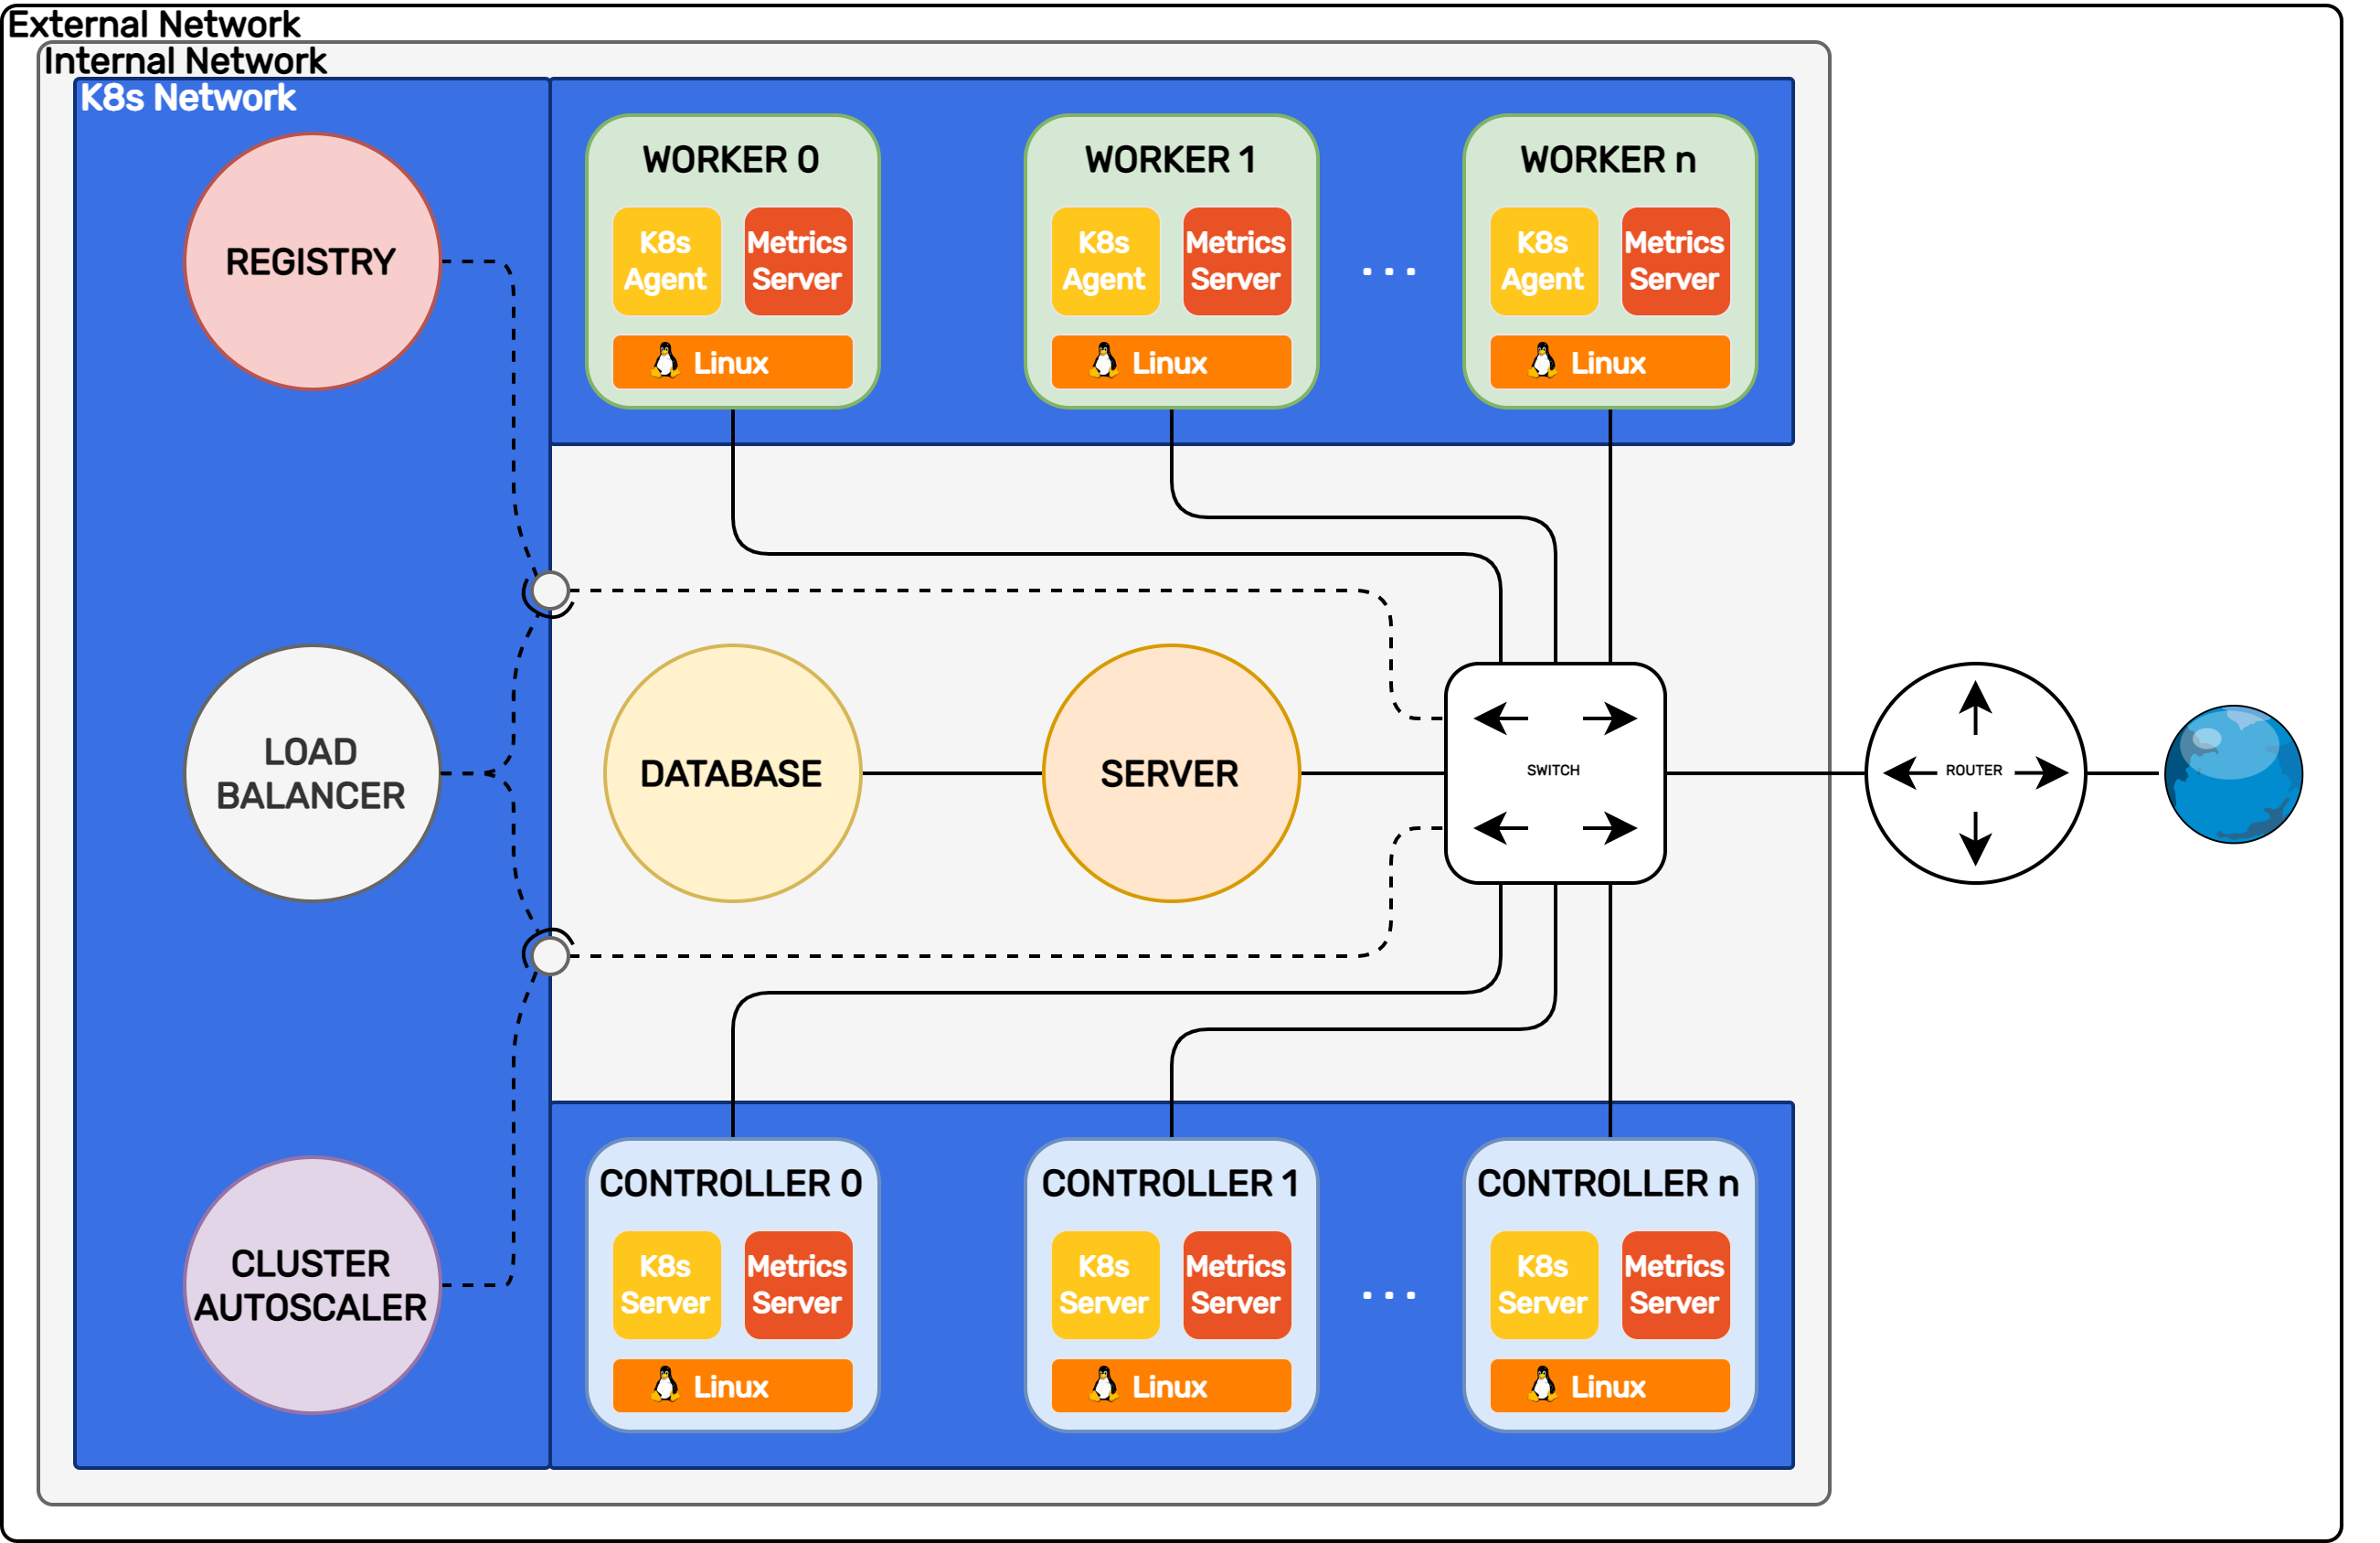
\includegraphics[width=.9\textwidth]{images/recluster/architecture.png}
  \caption{Architecture overview}
\end{figure}

\section{Components}
\label{sec:architecture_components}

\subsection{Node}
\label{subsec:architecture_components_node}

A node is a physical computer that runs the \texttt{Linux Kernel} and constantly
executes software that is specific to the cluster's composition. Linux is a
clone of the operating system Unix\footnote{\url{https://unix.org}}, written from
scratch by Linus Torvalds\footnote{\url{https://wikipedia.org/wiki/Linus_Torvalds}}
with help from a loosely-knit team of hackers across the world. It aims towards
POSIX and Single UNIX Specification compliance\cite{linux}.\\ %
Each node is physically connected to the other nodes via Ethernet and to the
many operating services/components through a virtual network. Section \ref{sec:architecture_network}
goes into further detail about cluster networking. \\ %
A node can be in one of two states. The \texttt{active} state indicates that a node
is turned on and is actively contributing to the cluster. The \texttt{inactive} state,
on the other hand, shows that a node has been turned off and is no longer actively
contributing to the cluster. This does not imply that the node is worthless and
will never be utilized again, but simply that it is no longer required for the current
cluster demand. A node state can be changed manually by switching the power
button on or off, or automatically through the Cluster Autoscaler component,
which monitors the current cluster state. More details about Cluster Autoscaler may
be found in section \ref{subsec:architecture_components_cluster_autoscaler}. \\ %
% TODO Maybe K8s reference section ?
Two core services are continuously operating on each node. The first service is
a Kubernetes-compliant distribution. Kubernetes, also known as K8s, is an open-source
solution for automating containerized application deployment, scaling, and administration\cite{k8s}.
The second service, Metrics Server, is a server that constantly monitors the node,
exposing hardware and operating system metrics. \\ %
Finally, each node is conceptually divided into two types depending on its role in
the cluster: Worker nodes and Controller nodes. These are discussed in the sections
that follow.

\subsubsection{Worker}
\label{subsubsec:architecture_components_node_worker}

\begin{wrapfigure}
  {l}{0pt} %
  \raisebox{0pt}[\dimexpr\height-\baselineskip\relax]{\centering
  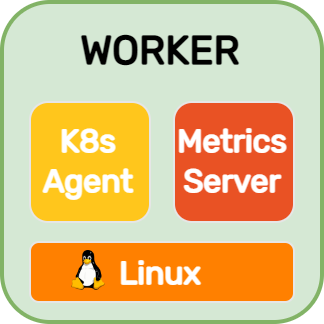
\includegraphics[width=.2\textwidth]{images/recluster/worker.png}}
\end{wrapfigure}

A worker node is designed to handle only deployable units of computation and services
that are not critical components of the cluster. It is not in charge of
scheduling the work over several nodes; rather, it only accepts it from a
cluster-available authenticated and authorized controller node. \\ %
Even though a worker node executes the effectively scheduled workload in the
cluster, it is not considered a critical component of it. At any given time, the
total number of active workers might be zero. That is, there is no scheduled workload,
and previously worker nodes have been shut down automatically to prevent
precious resource waste that is no longer required. \\ %
The majority of the cluster's accessible machines are worker nodes. This raises the
overall amount of schedulable workload as well as heterogeneity. Heterogeneity
is helpful because it may help schedule workloads to nodes with the bare minimum
of requested resources, preventing waste. Assume that the total number of
\texttt{active} nodes in the cluster is zero and that there are two \texttt{inactive}
worker nodes. The first node has 4 GiB of memory and consumes 100W of power,
whereas the second node has 8 GiB of memory and consumes 150W of power. A workload
using around 3GiB of memory is then planned for the cluster. Because it
decreases resource waste, notably memory waste, the first worker node will be
chosen. It is important to note that if both nodes have an equal amount of memory,
the conclusion remains the same since it has the lowest power consumption.

\subsubsection{Controller}
\label{subsubsec:architecture_components_node_controller}

\begin{wrapfigure}
  {l}{0pt} %
  \raisebox{0pt}[\dimexpr\height-\baselineskip\relax]{\centering
  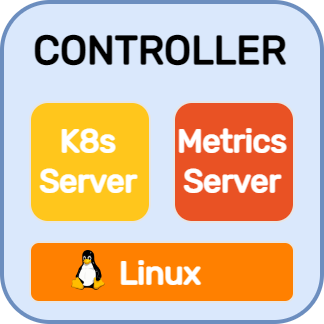
\includegraphics[width=.2\textwidth]{images/recluster/controller.png}}
\end{wrapfigure}

A controller node is an essential component of the cluster, acting as a coordinator
between the active worker nodes and the overall workload in the cluster. It
continually monitors the cluster's state in terms of available nodes, how and where
the workload should be scheduled, and much more. A consistent and secure API must
be provided for administration and end-users who wish to deploy custom services in
the cluster. The API can be made available to an external network if it is
available and appropriately configured, allowing remote control and improving overall
usage. \\ %
To ensure the integrity and management of a cluster, at least one controller
node must be constantly available. It is strongly suggested to have multiple controller
nodes that meet the high availability model to withstand potential system,
component, or application failures. This is possible considering an odd number
of controller nodes (i.e. three) that are always active. A quorum of controller
nodes is required for a cluster to agree on cluster state updates. Quorum in a cluster
with \texttt{n} controllers is \texttt{(n / 2) + 1}. Adding one node to any odd-sized
controller group will always increase the number of nodes required for a quorum.
Although adding a node to an odd-sized controller group appears to improve fault
tolerance since there are more machines, it worsens it because the same number
of nodes can crash without losing quorum but there are more nodes that can fail.
If the cluster cannot withstand any more failures, adding a node before removing
nodes is dangerous because if the new controller node fails to register, the cluster
quorum would be permanently lost\cite{quorum}. The latter is not a strict necessity,
but rather a preferable practice, even though it may slightly increase total resource
waste. Consider this: if the only available controller node encounters a software
or hardware failure and becomes unavailable, the entire cluster becomes
unreachable and unusable.\\ %
To further decrease overall resource waste, a controller can also become a
worker at the same time. If the overall workload in the cluster is very low and non-zero,
having one worker and one controller active with minimal utilization at the same
time is a waste. A single machine can perform the same task, saving precious
resources. If the entire demand grows later and the sole active node becomes overloaded,
the cluster reverts to its previous state. This is a configuration that may be enabled
or disabled based on the management needs of the cluster. \\ %
It should be noted that the total number of active or inactive nodes in the cluster
is not limited. However, a large number of nodes increases the workload on controller
nodes, which must maintain the cluster state updated and synchronized. As a result,
as shown in table \ref{tbl:controller_node_requirements}\cite{k3s_requirements},
their number and hardware requirements must be carefully balanced.

\begin{xltabular}
  {\textwidth} { c | >{\ttfamily}c | >{\ttfamily}c | >{\ttfamily}c }

  \multicolumn{1}{ c |}{\large{\textbf{Deployment Size}}} &
  \multicolumn{1}{ c |}{\large{\textbf{Nodes}}} &
  \multicolumn{1}{ c |}{\large{\textbf{CPU Cores}}} &
  \multicolumn{1}{ c}{\large{\textbf{RAM Memory}}} \\ \hline \hline

  Small & \raisebox{0.5ex}{\texttildelow}10 & 2 & 4 GiB \\ \hline

  Medium & \raisebox{0.5ex}{\texttildelow}100 & 4 & 8 GiB \\ \hline

  Large & \raisebox{0.5ex}{\texttildelow}250 & 8 & 16 GiB \\ \hline

  X-Large & \raisebox{0.5ex}{\texttildelow}500 & 16 & 32 GiB \\ \hline

  XX-Large & 500+ & 32 & 64 GiB \\

  \caption{Controller node requirements based on cluster size}
  \label{tbl:controller_node_requirements}
\end{xltabular}

\subsection{Server}
\label{subsec:architecture_components_server}

\begin{wrapfigure}
  {l}{0pt} %
  \raisebox{0pt}[\dimexpr\height-\baselineskip\relax]{\centering
  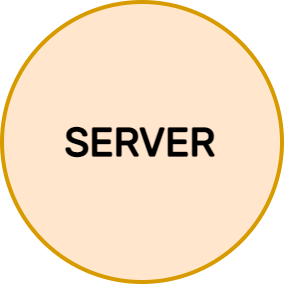
\includegraphics[width=.2\textwidth]{images/recluster/server.png}}
\end{wrapfigure}

A server handles all cluster nodes, user authentication and authorization, and much
more. It does not directly monitor the workload in the same way as a controller
node does, but it does serve as a low-level middleware controller. Every action
is made because of human intervention (e.g., administrators) or another
component of the cluster that has much higher-level knowledge of the current
state and reacts appropriately. \\ %
It is both an essential and a non-essential component of the cluster. It is essential
in the sense that it is aware of all registered nodes, both active and inactive,
and understands how to switch them on and off automatically. It reduces resource
waste by automatically increasing or decreasing the number of nodes in the
cluster when used in conjunction with the Cluster Autoscaler component (see section
\ref{subsec:architecture_components_cluster_autoscaler}). Without prior information,
there is no component in the cluster that can operate as an oracle about the
nodes, leaving the Cluster Autoscaler worthless and increasing total resource waste.
It is also deemed non-essential in the sense that, while decreasing resource waste
is the overall architecture's goal, there is no requirement for a high
availability model as in controller nodes. If a server instance crashes and does
not restart, leaving no more servers in the cluster, the entire cluster continues
to function normally. However, unless failures, human interaction, or server restarts,
the number of active nodes remains constant, potentially increasing resource waste.
\\ %
A server instance does not have to run on a dedicated node. A node can hold
numerous components at the same time, as previously mentioned. A node may be a
server, a controller, and a worker all at the same time, drastically decreasing resource
waste. It is crucial to note, however, that a server should not be executed on a
worker node since, as previously explained, the total number of active workers
might be zero, terminating the server instance and the capability of automatically
adjusting the cluster size. \\ %
The server provides an API to facilitate cluster administration. Furthermore, as
previously said, it is in charge of user authentication and authorization. Unharmful
queries (providing information about active nodes or listing non-sensible
information about a user) should not require any authentication or only a minimal
one. Queries that mutate the state of the cluster or display sensitive
information (turning on or off a node or displaying sensitive user information)
must be protected by a high-security mechanism. \\ %
A heartbeat daemon must be implemented on the server to continuously check the
condition of a node and detect any problems. A heartbeat is a periodic signal or
message created by hardware or software that is sent between devices at regular intervals
of seconds. If the endpoint does not receive a heartbeat for an extended period,
often many heartbeat intervals, the machine that should have sent the heartbeat
is assumed to have failed\cite{heartbeat}. The latter is commonly implemented by
controller nodes since they must constantly monitor and acquire information
about active nodes for workload scheduling. As a result, a server can use the
controller's API to eliminate duplication, increase consistency and availability,
and simplify implementation. \\ %
For more information, section \ref{sec:implementation_server} covers in detail how
the server component is implemented.

\subsection{Database}
\label{subsec:architecture_components_server_database}

\begin{wrapfigure}
  {l}{0pt} %
  \raisebox{0pt}[\dimexpr\height-\baselineskip\relax]{\centering
  
\includegraphics[width=.2\textwidth]{images/recluster/database.png}}
\end{wrapfigure}

The database component is strictly related to the server component. Its primary
function is to store all cluster-related data in a safe, persistent and fault-tolerant
system. The data in question is generally static and does not change frequently.
Static data includes all node-related information, such as CPU type and RAM
quantity, that is hardly modified after the node is added to the cluster.
However, some data, like information regarding the current node state and its
last heartbeat, are intrinsically dynamic in the sense that the system regularly
changes them to ensure integrity. Like the server component, is seen as both necessary
and non-essential. A server is worthless without the database, resulting in the same
outcome as previously explained. \\ %
This component is seen as the union of numerous modules that form it rather than
as a single entity. A database, in general, is a structured collection of
information or data that is persistently stored in a computer system. A database
management system (DBMS) is a software program that acts as an interface between
the database and its end users or applications, allowing for the retrieval, updating,
and administration of how information is structured and optimized. A DBMS also facilitates
database supervision and control by providing several administrative operations such
as performance monitoring, tuning, and backup and recovery\cite{database}. The latter
indicates that each module and feature is dependent on the implementation. Only
for the database itself, there are several distinct types, and for each type, there
are numerous distributions with varying features and capabilities. To better
follow the overall design criteria, the ultimate decision on which one to take must
be carefully examined. \\ %
Persistency and fault tolerance are strongly related, most importantly, in the data
layer. Even if an error occurs, the only vital and critical component that must be
preserved and not lost is all the stored data. Data persistency is the
preservation of data after the program that produced it has been terminated. To do
this, the data must be written to non-volatile storage, a type of memory that can
maintain the information indefinitely even if the program is no longer functioning\cite{persistency}.
Fault tolerance, which differs slightly from the previous definition, refers to a
non-volatile storage system's capacity to recover from an error or faulty condition,
most typically an irreversible hardware failure of some type, without losing any
previously stored data. Disk fault tolerance is often achieved by disk
management technologies such as mirroring\footnote{\url{https://wikipedia.org/wiki/Disk_mirroring}},
data striping\footnote{\url{https://wikipedia.org/wiki/Data_striping}},
duplexing\footnote{\url{https://www.pcmag.com/encyclopedia/term/disk-duplexing}},
and Redundant Array of Independent (or Inexpensive) Disks (RAID)\footnote{\url{https://wikipedia.org/wiki/RAID}}\cite{disk_management_technologies}.
Consider the possibility that the database component has a hardware failure and ceases
to operate. The damage has compromised not just the replaceable hardware (such as
the CPU, motherboard, and RAM), but also some (but not all) storage devices storing
the cluster's data. Typically, all data is irreversibly lost, and the cluster
must be rebuilt from scratch. However, with a correctly designed disk management
system, once the faulty hardware is replaced, all data is automatically
recovered and the cluster becomes functional again. The process of rebuilding the
data might take a significant amount of time (i.e. calculating the parity bit\footnote{\url{https://wikipedia.org/wiki/Parity_bit}}).
\\ %
Finally, an optional cache middleware can be implemented between the server and database,
enhancing read speed for frequently requested but rarely updated data and
reducing disk utilization. The cached data is stored in the main volatile memory.

\subsection{Registry}
\label{subsec:architecture_components_registry}

\begin{wrapfigure}
  {l}{0pt} %
  \raisebox{0pt}[\dimexpr\height-\baselineskip\relax]{\centering
  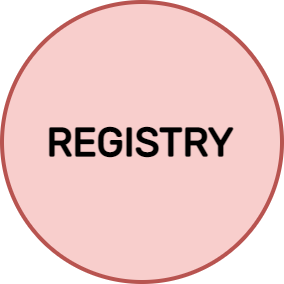
\includegraphics[width=.2\textwidth]{images/recluster/registry.png}}
\end{wrapfigure}

% TODO Air-Gap reference
% TODO Container reference

The registry component is a private container registry that the K8s orchestrator
uses in the cluster to download a specific image or collection of images. A container
registry is a stateless, highly scalable server-side application that stores and
distributes container-based application images\cite{container_registry}. \\ %
A registry is regarded as a non-essential component because the whole system may
function without it. If an internet connection is available and one of the
numerous public container registries (such as Docker Hub\footnote{\url{https://hub.docker.com}})
is accessible, the cluster downloads and runs the requested image from the external
network. Having a private register in the cluster, on the other hand, may solve
a plethora of potential difficulties. Some of them are as follows:

\begin{itemize}
  \item The K8s orchestrator fails to download the requested images in an Air-Gapped
    environment when there is no internet connection. As a result, the entire cluster
    is nearly unusable. The only realistic approach is to make a local duplicate
    of the remote images for each cluster node. This is hard to accomplish and prone
    to errors. Furthermore, there is a waste of disk memory, but it also ignores
    how and where the images are downloaded.

  \item A local solution is required for an organization that wants complete control
    over its images and is unwilling to put them on an external service.
    Furthermore, if the organization takes a security-first approach, a properly
    configured private registry can improve overall security.

  \item A newly developed image that must be evaluated before begin release to production.
    Moreover, the registry may be used to improve DevOps techniques by preventing
    potential bugs, security vulnerabilities, and other difficulties that can arise
    in a real-world environment. Attachment \ref{cha:good_practices} goes into
    much depth about DevOps.

  \item An image created exclusively for the cluster. Uploading it to a public
    registry is not only pointless due to incompatibility, but it also limits the
    available namespace because an image name must be unique.

  \item Registry as a pull-through cache\footnote{\url{https://docs.docker.com/registry/recipes/mirror}}.
    If multiple cluster nodes require the same external image and it does not
    exist locally, each of them fetches it from the specified registry. This
    results in excessive and inefficient network utilization, which might congest
    the cluster. The private registry can act as a registry mirror, locally caching
    each externally requested image. Every node points directly to the private
    registry address. If an image cannot be located locally, the request is
    routed to the local registry, which downloads and caches it. When a node
    requests the same image again, the registry provides the cached image without
    needing any further network traffic.
\end{itemize}

In practice, the registry is used to distribute the Cluster Autoscaler image (see
\ref{subsec:architecture_components_cluster_autoscaler}) that is specifically built
to function with reCluster. \\ %
Even though it is supported out of the box, the component does not need to be
instantiated on a specific physical node; rather, it is deployed directly in the
K8s environment. The registry may be accessible from both inside and outside the
K8s network, thanks to a correctly configured Load Balancer component (further information
in section \ref{subsec:architecture_components_load_balancer}) that exposes the
service to a non-K8s-related external network. Exposing the K8s service is critical
for conveniently allowing the upload (push) and download (pull) of an image without
the user requiring any extra settings. The approach must remain the same as when
utilizing a publicly accessible registry, but with the cluster's registry address
provided. Because the registry is externally accessible, it must be properly configured
to improve overall security. HTTPS\footnote{\url{https://wikipedia.org/wiki/HTTPS}},
which enables secure communication over a cryptographic channel, and
authentication, which permits access only to a limited group of authenticated users,
must be set up and/or implemented. \\ %
The registry is deployed in the K8s environment, but the K8s orchestrator needs it
to fetch the required images, leading to a circular dependence. To avoid the latter,
the registry image should be made available on each node, eliminating the need for
a registry request.

\subsection{Cluster Autoscaler}
\label{subsec:architecture_components_cluster_autoscaler}

\begin{wrapfigure}
  {l}{0pt} %
  \raisebox{0pt}[\dimexpr\height-\baselineskip\relax]{\centering
  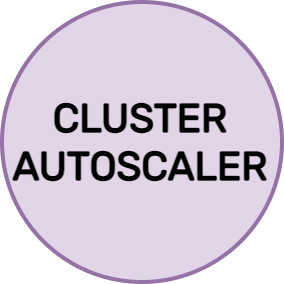
\includegraphics[width=.2\textwidth]{images/recluster/cluster_autoscaler.png}}
\end{wrapfigure}

\subsection{Load Balancer}
\label{subsec:architecture_components_load_balancer}

\begin{wrapfigure}
  {l}{0pt} %
  \raisebox{0pt}[\dimexpr\height-\baselineskip\relax]{\centering
  
\includegraphics[width=.2\textwidth]{images/recluster/load_balancer.png}}
\end{wrapfigure}

\section{Network}
\label{sec:architecture_network}

\subsection{Overlay Network}
\label{subsec:architecture_network_overlay_network}

\subsection{Domain}
\label{subsec:architecture_network_domain}

\section{Cluster}
\label{sec:architecture_cluster}

\begin{wrapfigure}
  {r}{.5\textwidth}
  \centering
  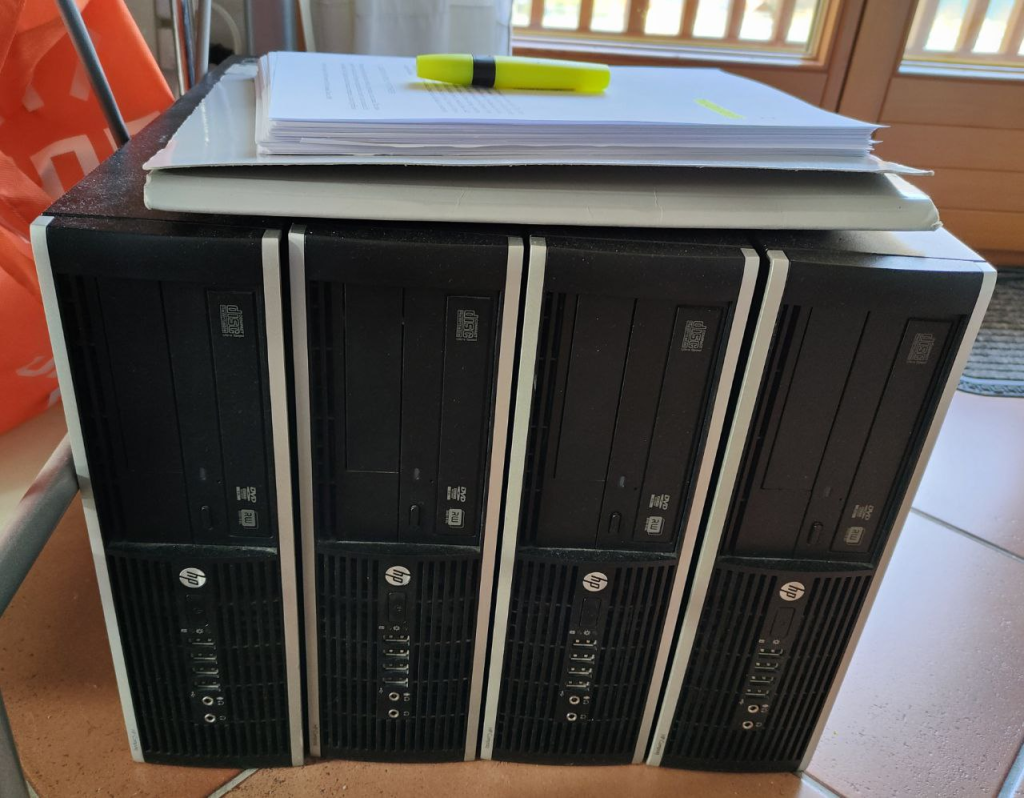
\includegraphics[width=.5\textwidth]{images/recluster/cluster.png}
  \caption{reCluster cluster}
\end{wrapfigure}

\subsection{Hardware}
\label{subsec:architecture_cluster_hardware}

% TODO WoL features, how to turn on nodes
% TODO Prefer nodes with WoL upscaling

\subsection{Example}
\label{subsec:architecture_cluster_example}

% TODO Move